% Name: Deployment diagram
% Description: A UML deployment diagram: the browser, an application server running the web app, and a database server, drawn as 3D nodes with the artifacts deployed on them.
% Tags: deployment diagram, UML, nodes, artifacts

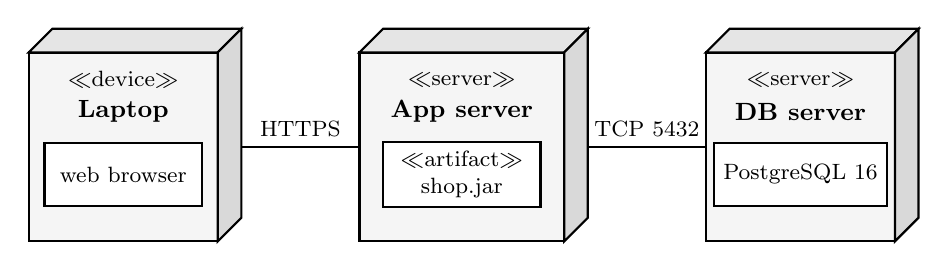
\begin{tikzpicture}[thick, every node/.style={font=\small},
    artifact/.style={draw, fill=white, minimum width=20mm, minimum height=8mm, font=\footnotesize, align=center}]
  % A node is a box with a top and a side face, offset by (0.3, 0.3).
  \foreach \x/\w/\name/\kind in {0/2.4/client/device, 4.2/2.6/app/server, 8.6/2.4/db/server} {
    \draw[fill=gray!8] (\x,0) rectangle ++(\w,2.4);
    \draw[fill=gray!20] (\x,2.4) -- ++(0.3,0.3) -- ++(\w,0) -- ++(-0.3,-0.3) -- cycle;
    \draw[fill=gray!30] (\x+\w,0) -- ++(0.3,0.3) -- ++(0,2.4) -- ++(-0.3,-0.3) -- cycle;
    \node[font=\footnotesize] at (\x+\w/2,2.05) {$\ll$\kind$\gg$};
    \coordinate (\name) at (\x+\w/2,0.85);
  }
  \node at ([yshift=8mm]client) {\textbf{Laptop}};
  \node at ([yshift=8mm]app) {\textbf{App server}};
  \node at ([yshift=8mm]db) {\textbf{DB server}};
  \node[artifact] (a1) at (client) {web browser};
  \node[artifact] (a2) at (app) {$\ll$artifact$\gg$\\shop.jar};
  \node[artifact] (a3) at (db) {PostgreSQL 16};
  \draw (2.7,1.2) -- node[above, font=\footnotesize] {HTTPS} (4.2,1.2);
  \draw (7.1,1.2) -- node[above, font=\footnotesize] {TCP 5432} (8.6,1.2);
\end{tikzpicture}
